\documentclass[11pt,a4paper]{article}

% ---------------------------------------------------------------------------
% Packages
% ---------------------------------------------------------------------------
\usepackage[utf8]{inputenc}
\usepackage[T1]{fontenc}
\usepackage{lmodern}
\usepackage[margin=2.5cm]{geometry}
\usepackage{amsmath,amssymb}
\usepackage{graphicx}
\usepackage{booktabs}
\usepackage{array}
\usepackage{multirow}
\usepackage{caption}
\usepackage{subcaption}
\usepackage{float}
\usepackage{enumitem}
\usepackage{xcolor}
\usepackage{listings}
\usepackage[hidelinks]{hyperref}

\graphicspath{{figures/}}
% Shared style for all PGFPlots figures of the report.
% Load it in the preamble with:  % Shared style for all PGFPlots figures of the report.
% Load it in the preamble with:  % Shared style for all PGFPlots figures of the report.
% Load it in the preamble with:  \input{pgf_figures/style}
% The figures read their data from report/data/*.csv (paths relative to the report folder).
\usepackage{pgfplots}
\usepackage{pgfplotstable}
\usepgfplotslibrary{groupplots}
\pgfplotsset{compat=1.18}

% One colour per method, used consistently in every figure.
\definecolor{layerwise}{HTML}{7B4F9E}   % layer-wise L1 pruning (Ex. 1-2)
\definecolor{global}{HTML}{14837B}      % global L1 pruning (Ex. 3)
\definecolor{finetuned}{HTML}{D9692E}   % global pruning + re-training (Ex. 4)
\definecolor{iterative}{HTML}{2E4A6B}   % iterative pruning + re-training (Ex. 5)
\definecolor{structured}{HTML}{C2477A}  % structured filter pruning (Bonus)
\definecolor{refgray}{HTML}{555555}     % baseline / reference lines

\newcommand{\baselineacc}{68.67}  % baseline validation accuracy (%)

\pgfplotsset{
  report/.style={
    width=\linewidth, height=6cm,
    grid=major, grid style={gray!20},
    axis line style={gray!60},
    xtick pos=bottom, ytick pos=left,
    tick label style={font=\small},
    label style={font=\small},
    legend style={font=\small, draw=none, fill=white, fill opacity=0.85, text opacity=1},
    legend cell align=left,
    every axis plot/.append style={line width=1.1pt},
    mark size=1.8pt,
    table/col sep=comma,
  },
  % Legend placed under the plot, for figures with many curves.
  legend below/.style={
    legend style={at={(0.5,-0.27)}, anchor=north, legend columns=#1, /tikz/every even column/.append style={column sep=0.6em}},
  },
  legend below/.default=3,
  % Horizontal reference lines.
  baseline line/.style={refgray, dashed, line width=0.8pt, mark=none},
  chance line/.style={refgray!70, dotted, line width=0.8pt, mark=none},
}

% The figures read their data from report/data/*.csv (paths relative to the report folder).
\usepackage{pgfplots}
\usepackage{pgfplotstable}
\usepgfplotslibrary{groupplots}
\pgfplotsset{compat=1.18}

% One colour per method, used consistently in every figure.
\definecolor{layerwise}{HTML}{7B4F9E}   % layer-wise L1 pruning (Ex. 1-2)
\definecolor{global}{HTML}{14837B}      % global L1 pruning (Ex. 3)
\definecolor{finetuned}{HTML}{D9692E}   % global pruning + re-training (Ex. 4)
\definecolor{iterative}{HTML}{2E4A6B}   % iterative pruning + re-training (Ex. 5)
\definecolor{structured}{HTML}{C2477A}  % structured filter pruning (Bonus)
\definecolor{refgray}{HTML}{555555}     % baseline / reference lines

\newcommand{\baselineacc}{68.67}  % baseline validation accuracy (%)

\pgfplotsset{
  report/.style={
    width=\linewidth, height=6cm,
    grid=major, grid style={gray!20},
    axis line style={gray!60},
    xtick pos=bottom, ytick pos=left,
    tick label style={font=\small},
    label style={font=\small},
    legend style={font=\small, draw=none, fill=white, fill opacity=0.85, text opacity=1},
    legend cell align=left,
    every axis plot/.append style={line width=1.1pt},
    mark size=1.8pt,
    table/col sep=comma,
  },
  % Legend placed under the plot, for figures with many curves.
  legend below/.style={
    legend style={at={(0.5,-0.27)}, anchor=north, legend columns=#1, /tikz/every even column/.append style={column sep=0.6em}},
  },
  legend below/.default=3,
  % Horizontal reference lines.
  baseline line/.style={refgray, dashed, line width=0.8pt, mark=none},
  chance line/.style={refgray!70, dotted, line width=0.8pt, mark=none},
}

% The figures read their data from report/data/*.csv (paths relative to the report folder).
\usepackage{pgfplots}
\usepackage{pgfplotstable}
\usepgfplotslibrary{groupplots}
\pgfplotsset{compat=1.18}

% One colour per method, used consistently in every figure.
\definecolor{layerwise}{HTML}{7B4F9E}   % layer-wise L1 pruning (Ex. 1-2)
\definecolor{global}{HTML}{14837B}      % global L1 pruning (Ex. 3)
\definecolor{finetuned}{HTML}{D9692E}   % global pruning + re-training (Ex. 4)
\definecolor{iterative}{HTML}{2E4A6B}   % iterative pruning + re-training (Ex. 5)
\definecolor{structured}{HTML}{C2477A}  % structured filter pruning (Bonus)
\definecolor{refgray}{HTML}{555555}     % baseline / reference lines

\newcommand{\baselineacc}{68.67}  % baseline validation accuracy (%)

\pgfplotsset{
  report/.style={
    width=\linewidth, height=6cm,
    grid=major, grid style={gray!20},
    axis line style={gray!60},
    xtick pos=bottom, ytick pos=left,
    tick label style={font=\small},
    label style={font=\small},
    legend style={font=\small, draw=none, fill=white, fill opacity=0.85, text opacity=1},
    legend cell align=left,
    every axis plot/.append style={line width=1.1pt},
    mark size=1.8pt,
    table/col sep=comma,
  },
  % Legend placed under the plot, for figures with many curves.
  legend below/.style={
    legend style={at={(0.5,-0.27)}, anchor=north, legend columns=#1, /tikz/every even column/.append style={column sep=0.6em}},
  },
  legend below/.default=3,
  % Horizontal reference lines.
  baseline line/.style={refgray, dashed, line width=0.8pt, mark=none},
  chance line/.style={refgray!70, dotted, line width=0.8pt, mark=none},
}
  % style of the PGFPlots figures (pgf_figures/*.tex)
\setlength{\parskip}{0.4em}
\captionsetup{font=small,labelfont=bf}

\lstset{
  language=Python,
  basicstyle=\ttfamily\footnotesize,
  keywordstyle=\color{blue!60!black}\bfseries,
  commentstyle=\color{green!40!black}\itshape,
  stringstyle=\color{red!50!black},
  frame=single,
  rulecolor=\color{black!30},
  breaklines=true,
  showstringspaces=false,
  columns=fullflexible
}

\newcommand{\code}[1]{\texttt{#1}}

% ---------------------------------------------------------------------------
% Cover page details: edit them here.
\newcommand{\studentname}{Gourab Roy}
\newcommand{\githublink}{https://github.com/GourabRoy551/cifar100-pruning-lab}

\begin{document}

% ---------------------------------------------------------------------------
% Cover page
% ---------------------------------------------------------------------------
\begin{titlepage}
\centering
\vspace*{1.5cm}
{\Large\scshape Universit\'e de Bordeaux\par}
\vspace{0.4cm}
{\large Master IPCV --- Academic Year 2026--2027\par}
\vspace{0.2cm}
{\large Advanced Topics in Image Processing and Computer Vision\par}

\vspace{2cm}
\rule{\linewidth}{0.8pt}\par
\vspace{0.5cm}
{\large\scshape Lab 1\par}
\vspace{0.4cm}
{\huge\bfseries Pruning a ResNet-18-like Network\\[0.2cm] on CIFAR-100\par}
\vspace{0.5cm}
{\Large Layer-wise, Global, Iterative and Structured Pruning in PyTorch\par}
\vspace{0.5cm}
\rule{\linewidth}{0.8pt}\par

\vfill
\begin{tabular}{@{}ll@{}}
\textbf{Student:} & \studentname \\[0.3em]
\textbf{Code:}    & \expandafter\url\expandafter{\githublink} \\[0.3em]
\textbf{Date:}    & October 2026 \\
\end{tabular}
\vspace{2.5cm}
\end{titlepage}

\tableofcontents
\newpage

% ===========================================================================
\section{Introduction}
% ===========================================================================

In this lab I used the \code{torch.nn.utils.prune} package of PyTorch to prune a convolutional network trained on CIFAR-100. I wanted to find out how many weights I could remove before the accuracy dropped too much, which way of choosing the weights works best, and whether re-training can repair the damage. I first trained my own compact ResNet-18-like network (2.82\,M parameters), which reached 68.67\% validation and 68.54\% test accuracy. I then went through the exercises in order: layer-by-layer pruning (Exercises~1--2), global pruning (Exercise~3), re-training of the pruned models (Exercise~4), iterative pruning (Exercise~5) and, as a bonus, my own structured pruning method. At the end I evaluated the selected models once on the test set.

\textbf{My main finding is that \emph{where} the weights are removed, and whether the network can re-adapt, matter much more than \emph{how many} are removed.} Layer-by-layer pruning lost 42 points at only 20\% sparsity, while global pruning removed half of the weights while staying within one point of the baseline. After five epochs of re-training, \textbf{my final model has 70\% of its weights removed and reaches 68.34\% test accuracy}, only 0.20 points below the baseline. Iterative pruning did not improve on this except at 90\% sparsity, and my structured method cost more accuracy but is the only one whose zeros could make the network really smaller. Figure~\ref{fig:overview} summarises these results.

\begin{figure}[H]
\centering
% Figure 1: overview of all pruning methods (validation accuracy vs sparsity).
\begin{tikzpicture}
\begin{axis}[report, legend below=3,
  xlabel={Sparsity (\%)}, ylabel={Validation accuracy (\%)},
  xmin=-2, xmax=92, ymin=0, ymax=85, xtick={0,10,...,90}, ytick={0,20,...,80}]
\addplot[layerwise, mark=*] table[x=sparsity, y=acc]{data/ex2.csv};
\addlegendentry{Layer-wise (Ex.~2)}
\addplot[global, mark=square*] table[x=sparsity, y=acc]{data/ex3.csv};
\addlegendentry{Global (Ex.~3)}
\addplot[finetuned, mark=triangle*] table[x=sparsity, y=after]{data/ex4.csv};
\addlegendentry{Global + re-training (Ex.~4)}
\addplot[iterative, mark=diamond*] table[x=sparsity, y=after_retraining]{data/ex5.csv};
\addlegendentry{Iterative + re-training (Ex.~5)}
\addplot[baseline line] coordinates {(-5,\baselineacc) (95,\baselineacc)};
\addlegendentry{Baseline (68.67\%)}
\node[circle, draw=finetuned!80!black, line width=1.2pt, minimum size=9pt, inner sep=0pt] (choice) at (axis cs:70,68.05) {};
\node[font=\small, text=finetuned!80!black, anchor=south] at (axis cs:70,72) {My choice: 70\%};
\end{axis}
\end{tikzpicture}

\caption{Overview of the validation accuracy of all pruning methods against sparsity. Each marker is a measured model; the circle marks my final choice.}
\label{fig:overview}
\end{figure}

% ===========================================================================
\section{Background}
% ===========================================================================

\subsection{What pruning means}
The way I understood pruning in this lab is simple: I take a trained network, set some of its weights to zero, and check how much accuracy it loses. The real question is \emph{which} weights to remove, and the lab describes this with three choices. The \textbf{granularity} says whether single weights are removed (\emph{unstructured}) or whole groups such as complete filters (\emph{structured})~\cite{li2017pruning}. The \textbf{scope} says whether the same percentage is removed in every layer (\emph{layer-wise}) or whether all weights are ranked together (\emph{global}). The \textbf{criterion} decides which weights are unimportant; in this lab it was always their absolute value (L1 norm)~\cite{han2015learning}. By \emph{sparsity} I mean the percentage of weights that are exactly zero.

In practice, removing a fraction of the weights with L1 pruning means choosing a threshold $\tau$ and removing every weight with $|w_i| \le \tau$. \textbf{With layer-wise pruning each layer gets its own threshold, with global pruning there is one threshold for the whole network.} At first this looked like a small detail to me, but it turned out to be the most important difference in the whole lab.

\subsection{How PyTorch implements pruning}
Before starting, I expected pruning to delete weights, but PyTorch~\cite{paszke2019pytorch,paganini2019pruning} does not do that. It keeps the original values in \code{weight\_orig}, adds a 0/1 buffer \code{weight\_mask}, and recomputes the weight used in each forward pass as
\begin{equation}
  \mathbf{W} = \mathbf{W}_{\text{orig}} \odot \mathbf{M}.
\end{equation}
This had two consequences for my code: \textbf{pruned weights stay at zero during re-training} as long as the mask is kept, because they receive no gradient, and \textbf{a model saved with its masks is twice as large}. \code{prune.remove} makes the pruning permanent and deletes the two extra tensors.

\subsection{Re-training and iterative pruning}
Pruning without any further training is called \emph{one-shot} pruning. From the course I knew that re-training after pruning should allow much higher sparsity~\cite{han2015learning}, and that \emph{iterative} pruning, repeating prune~$\rightarrow$~re-train with increasing sparsity~\cite{zhu2017prune}, is usually said to work better at high sparsity. I did not want to simply accept this, so checking it on my own model was one of my goals in Exercises~4 and~5.

% ===========================================================================
\section{Experimental Setup}
% ===========================================================================

\subsection{Data and protocol}
I used CIFAR-100~\cite{krizhevsky2009learning}, with 100 classes of $32\times32$ images. As the template asks, I split the 50{,}000 training images into 40{,}000 for training and 10{,}000 for validation, and kept the 10{,}000 official test images for the end. \textbf{I saved the split indices to a file} (\code{cifar100\_split.pt}) and reloaded them in every script, because the template warns that re-generating the split would leak validation images into training. The images are normalised to $[-1,1]$, and only the training images are augmented with random crops and horizontal flips.

\textbf{Every decision (best epoch, kept sparsity, final model) was made on the validation set; the test set was never used for any decision, I only report it.} Since Exercises~2--5 all ask which model I would keep, I fixed one rule in advance: \emph{keep the highest sparsity whose validation accuracy is at most one point below the baseline} ($\ge 67.67\%$).

\subsection{Implementation and environment}
I kept the structure of the lab templates: \code{train.py} for Exercise~0, \code{pruning.py} for Exercises~1--5 and the bonus, and an independent \code{evaluate.py} that re-evaluates any saved model, as recommended in the instructions. In \code{pruning.py} a switch runs one exercise at a time, and each exercise saves its models, results, log and figures, so later exercises load saved models instead of re-running earlier ones. Everything ran on an RTX~4060 laptop GPU with PyTorch~2.14 and a fixed seed (42). On 10{,}000 images, an accuracy near 68\% has a standard error of about $\sqrt{0.68 \times 0.32/10000} \approx 0.47$ points, so I do not over-interpret differences of a few tenths of a point.

% ===========================================================================
\section{Exercise 0: Building a Baseline}
% ===========================================================================

\subsection{Choice of architecture}
The lab recommends a ``large enough'' network such as ResNet-18 with fewer max-pooling layers, aiming at 65--70\%, and warns against a network that is too large to prune. My first attempt with the full torchvision ResNet-18 reached about 75.5\%, but with 11.2\,M parameters it was larger than needed, so \textbf{I wrote my own lighter network that keeps the ResNet-18 structure~\cite{he2016deep} with half its width} (32--64--128--256 channels). It has four stages of two basic blocks with batch normalisation~\cite{ioffe2015batch} and residual shortcuts, global average pooling and a linear classifier. The stem is a single $3\times3$ convolution with stride 1 and \textbf{no max-pooling}: on $32\times32$ images, the original $7\times7$ stride-2 convolution and max-pooling would reduce the resolution far too early. Removing this single max-pooling layer is how I applied the lab's advice to use ``ResNet-18 with less max pooling''; the resolution is still reduced by the stride-2 convolutions of stages 2--4 ($32 \rightarrow 16 \rightarrow 8 \rightarrow 4$). The model has \textbf{2{,}820{,}740 parameters}, and \textbf{stage~4 alone holds 74\% of them} (Table~\ref{tab:arch}), which matters later.

\begin{table}[H]
\centering
\caption{Architecture of the ResNet-18-like baseline and distribution of its parameters.}
\label{tab:arch}
\begin{tabular}{lcccr}
\toprule
Stage & Blocks & Channels & Output size & Parameters \\
\midrule
Stem (conv $3\times3$ + BN + ReLU) & -- & 32 & $32\times32$ & 928 \\
Stage 1 & 2 & 32 & $32\times32$ & 37{,}120 \\
Stage 2 & 2 & 64 & $16\times16$ & 131{,}712 \\
Stage 3 & 2 & 128 & $8\times8$ & 525{,}568 \\
Stage 4 & 2 & 256 & $4\times4$ & 2{,}099{,}712 \\
Average pooling + linear & -- & 100 & -- & 25{,}700 \\
\midrule
Total & & & & 2{,}820{,}740 \\
\bottomrule
\end{tabular}
\end{table}

\subsection{Training}
Following the template, I used the cross-entropy loss and SGD (learning rate 0.1, momentum 0.9, weight decay $5\times10^{-4}$, batch size 128) with a cosine learning-rate schedule~\cite{loshchilov2017sgdr}. Since my full-width attempt had overshot the target, I trained for only \textbf{30 epochs} (8.6 minutes). I kept the checkpoint with the best validation accuracy, plus a backup copy, since every later exercise starts from it.

\subsection{Results}

\begin{figure}[H]
\centering
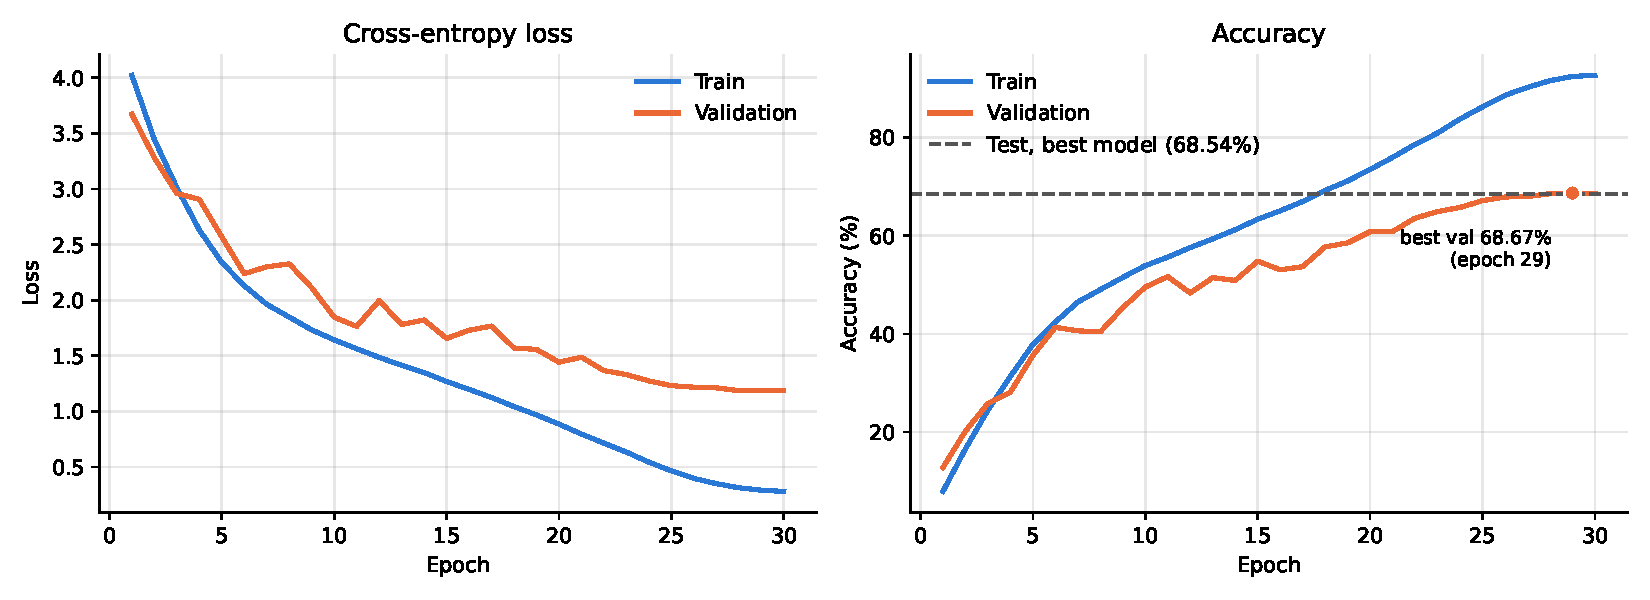
\includegraphics[width=\linewidth]{ex0_training_curves.pdf}
\caption{Exercise~0: training and validation loss (left) and accuracy (right). The dashed line is the test accuracy of the selected model.}
\label{fig:ex0}
\end{figure}

\textbf{The best checkpoint (epoch 29) reaches 68.67\% on validation and 68.54\% on the test set}, inside the 65--70\% range asked by the lab. The two accuracies differ by only 0.13 points, which reassured me that the saved split works as intended. The curves in Figure~\ref{fig:ex0} show two phases: while the learning rate is high, the validation accuracy progresses slowly and fluctuates, and in the last ten epochs, as the learning rate decays, it climbs steadily from about 61\% to 68.7\%. \textbf{The model clearly over-fits}: the training accuracy reaches 92.4\%, about 24 points above validation. This gap explains several observations in the later exercises.

% ===========================================================================
\section{Exercise 1: Pruning a Pre-trained Model}
% ===========================================================================

\subsection{What I implemented}
Following the three steps of the template, I collected all 41 layers that have parameters (20 convolutions, 20 batch-normalisation layers and the classifier), took their 62 weight and bias tensors, and pruned each of them at 20\% with \code{prune.l1\_unstructured}. Since the template says to prune \emph{all} layers with their biases, \textbf{I also pruned the batch-normalisation parameters}, a choice that turned out to matter. Printing \code{model.named\_buffers()} showed the 62 masks; one $3\times3$ kernel of the first convolution, for example, had one zero among nine entries, which made the mask mechanism very concrete for me. Finally I called \code{prune.remove}, the ``compression'' step of the template.

\subsection{Results}

\begin{figure}[H]
\centering
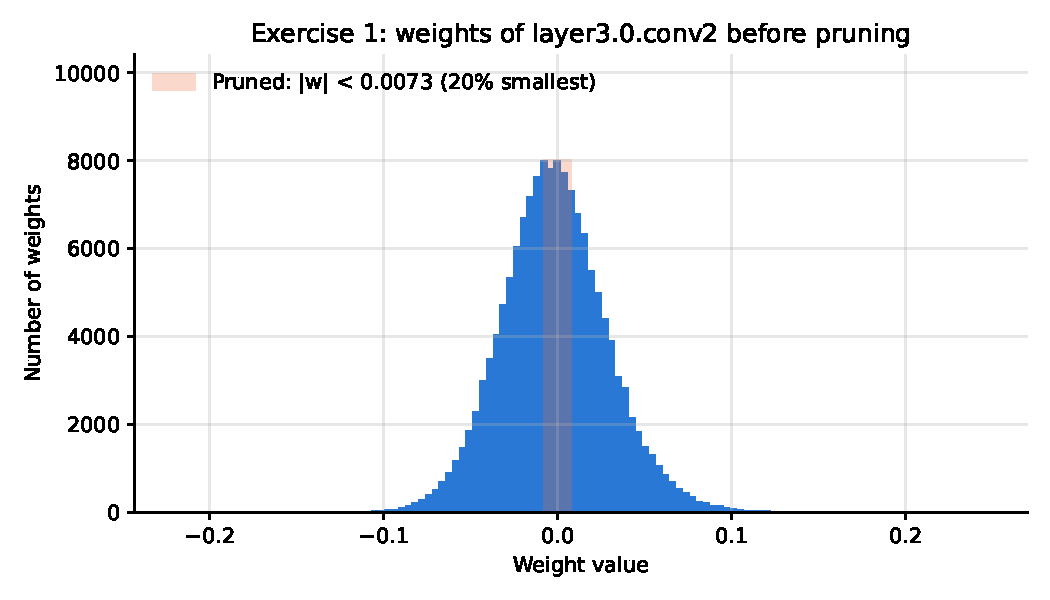
\includegraphics[width=0.7\linewidth]{ex1_weight_histogram.pdf}
\caption{Exercise~1: weights of \code{layer3.0.conv2} before pruning. The shaded band ($|w| \le 0.0073$) is what 20\% layer-by-layer L1 pruning removes.}
\label{fig:ex1}
\end{figure}

\begin{table}[H]
\centering
\caption{Exercise~1: effect of 20\% layer-by-layer pruning (validation set).}
\label{tab:ex1}
\begin{tabular}{lrr}
\toprule
 & Baseline & Pruned (20\%) \\
\midrule
Zero parameters & 0 & 564{,}148 (20.00\%) \\
Validation accuracy & 68.67\% & 26.73\% \\
Accuracy after \code{prune.remove} & -- & 26.73\% (identical) \\
File size, with masks / after \code{prune.remove} & 11.34\,MB & 22.65\,MB / 11.34\,MB \\
\bottomrule
\end{tabular}
\end{table}

Technically, the pruning behaved as intended: the sparsity is exactly 20.00\%, every layer lost about 20\% of its parameters, and the removed weights are those closest to zero (Figure~\ref{fig:ex1}). \textbf{The effect on accuracy, however, surprised me: removing only the 20\% smallest weights made the validation accuracy fall from 68.67\% to 26.73\%.} I first suspected a bug, but the sparsity was exact and the accuracy is identical after \code{prune.remove}, so the drop is a genuine property of this way of pruning.

My interpretation, which I develop in Exercises~2 and~3, is that \textbf{layer-by-layer pruning treats every layer the same, however sensitive it is}. The first convolution (864 weights) and the classifier are pruned as hard as the large stage-4 convolutions (up to 589{,}824 weights each). Pruning the batch-normalisation scales also matters: each scale multiplies a whole channel, so removing 20\% of them effectively switches off about 20\% of the channels everywhere. My compact model has little redundancy to lose; with the full-width ResNet-18, the same pruning cost about 27 points instead of 42.

\textbf{Pruning did not compress the file.} With its masks, the model takes twice the space of the baseline (22.65 vs 11.34\,MB), and after \code{prune.remove} it is back to exactly 11.34\,MB, not less, because the zeros are still stored in dense tensors. This was an important lesson for me: unstructured sparsity reduces the number of non-zero weights, but not the file size or the inference time. I return to this point in the bonus.

% ===========================================================================
\section{Exercise 2: Accuracy / Sparsity Ratio Curve}
% ===========================================================================

\subsection{What I implemented}
Following the template's tips, I moved the pruning of Exercise~1 into a function and applied it at 12 ratios (0, 5, 10, 15, 20, 30, \dots, 90\%), with finer steps below 20\% because I already knew that 20\% was harmful. Since pruning modifies the model in place, \textbf{I reloaded the original weights before every ratio}, evaluated on the same saved validation split, and saved each result and model immediately.

\subsection{Results}

\begin{figure}[H]
\centering
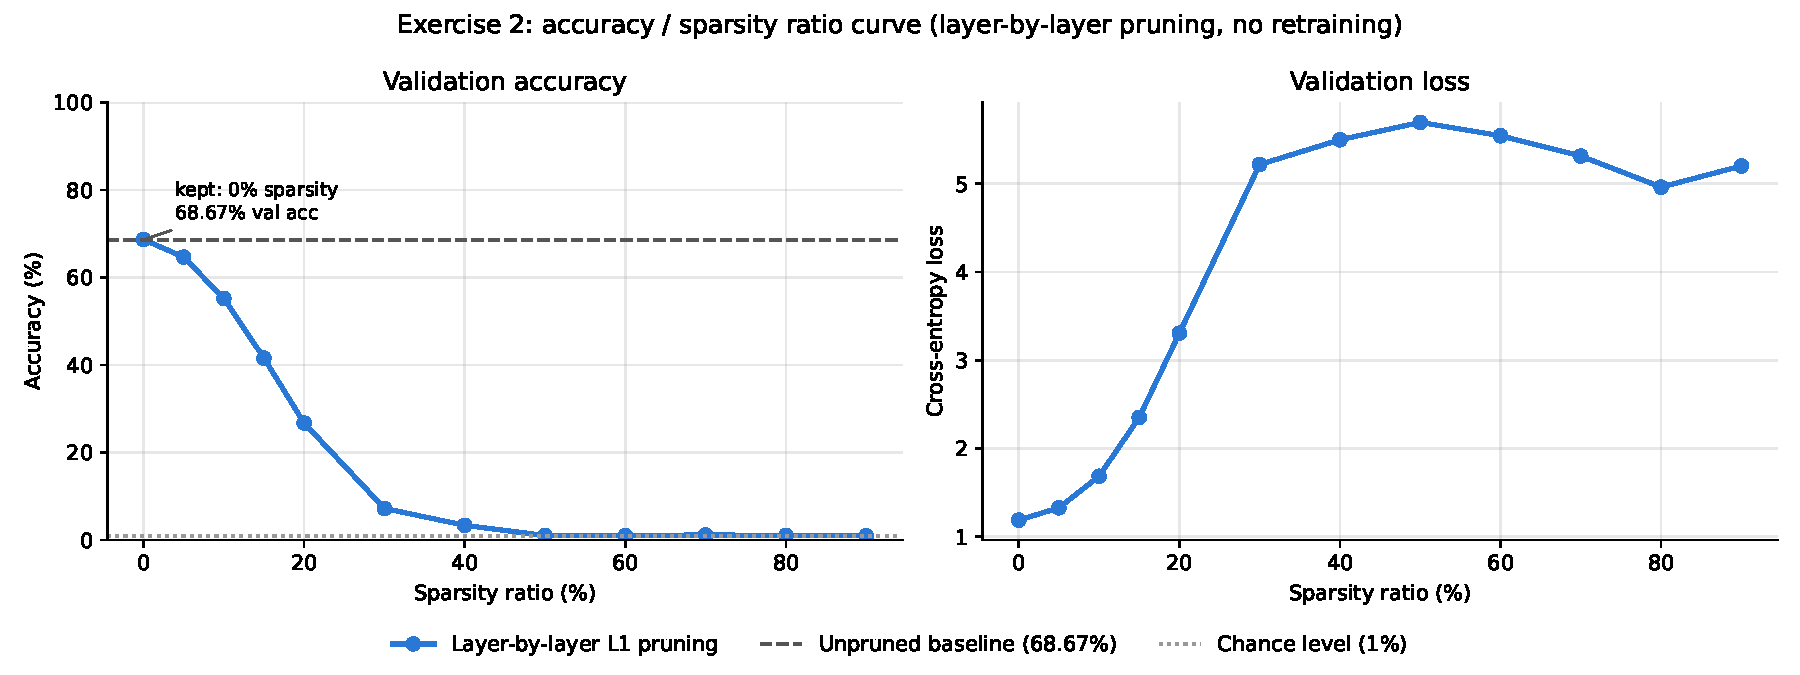
\includegraphics[width=\linewidth]{ex2_curve.pdf}
\caption{Exercise~2: layer-by-layer L1 pruning without re-training.}
\label{fig:ex2}
\end{figure}

\begin{table}[H]
\centering
\caption{Exercise~2: validation accuracy of layer-by-layer pruning.}
\label{tab:ex2}
\resizebox{\linewidth}{!}{%
\begin{tabular}{rrrrrrrrr}
\toprule
Sparsity & 0\% & 5\% & 10\% & 15\% & 20\% & 30\% & 40\% & 50--90\% \\
\midrule
Accuracy & 68.67\% & 64.66\% & 55.20\% & 41.57\% & 26.73\% & 7.22\% & 3.35\% & 0.95--1.17\% \\
\bottomrule
\end{tabular}}
\end{table}

\subsection{Comments on the curve}
\textbf{The curve has three clear regions}: a small but visible loss at 5\% (4 points), a collapse between 5\% and 30\%, and chance level (about 1\%) from 50\%. The 20\% point equals Exercise~1 exactly, which confirms that the weights were correctly reloaded. Beyond 30\%, the loss stays between about 5.0 and 5.7, above the $\ln(100) \approx 4.61$ of a uniform guess, so the pruned networks are not just uncertain but confidently wrong. \textbf{I think the problem is not the L1 criterion itself but its layer-wise use}: L1 ranks the weights correctly within a layer, but it cannot know that the first convolution, the classifier and batch normalisation are much more sensitive than the other layers. A variant that leaves batch normalisation unpruned would test this, but I did not run it.

\subsection{Which sparsity ratio would I keep, and why?}
Under my one-point rule, \textbf{I would keep 0\%}. Even 5\% costs four times the allowed loss, and since unstructured zeros do not shrink the model, losing 4 points for 5\% of zeros is not worth it. With a budget of about five points, 5\% would be the only reasonable choice.

% ===========================================================================
\section{Exercise 3: Global Pruning}
% ===========================================================================

\subsection{What I implemented}
I used \code{prune.global\_unstructured} with its three arguments: the same 62 (layer, name) tuples, \code{prune.L1Unstructured} as the method, and the sparsity ratio as \code{amount}. The protocol was the same as in Exercise~2, and following the template's tip, \textbf{I saved every model with its masks} so that Exercise~4 could re-train them.

\subsection{Results}

\begin{figure}[H]
\centering
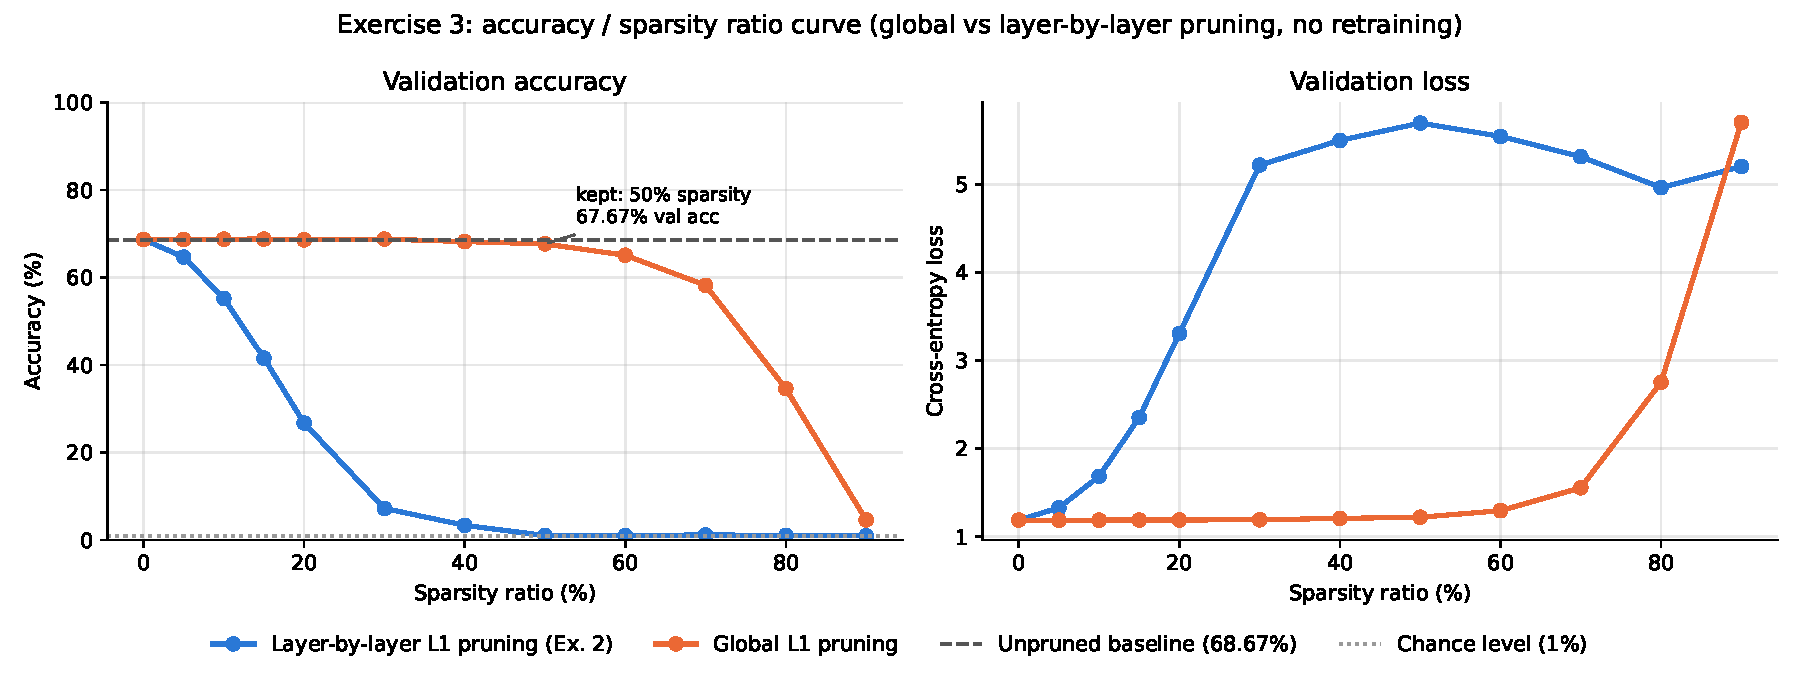
\includegraphics[width=\linewidth]{ex3_curve.pdf}
\caption{Exercise~3: global versus layer-by-layer L1 pruning, without re-training.}
\label{fig:ex3}
\end{figure}

\begin{table}[H]
\centering
\caption{Exercise~3: validation accuracy of global pruning compared with layer-wise pruning.}
\label{tab:ex3}
\resizebox{\linewidth}{!}{%
\begin{tabular}{rrrrrrrrrr}
\toprule
Sparsity & 10\% & 20\% & 30\% & 40\% & \textbf{50\%} & 60\% & 70\% & 80\% & 90\% \\
\midrule
Global & 68.77\% & 68.61\% & 68.78\% & 68.21\% & \textbf{67.67\%} & 65.09\% & 58.22\% & 34.60\% & 4.61\% \\
Layer-wise (Ex.~2) & 55.20\% & 26.73\% & 7.22\% & 3.35\% & 1.03\% & 0.99\% & 1.17\% & 1.04\% & 0.95\% \\
\bottomrule
\end{tabular}}
\end{table}

\subsection{Comments on the curve}
\textbf{The difference with Exercise~2 is striking: at 50\% sparsity, layer-wise pruning is at chance level while global pruning still gives 67.67\%.} Up to 50\% the global model stays within one point of the baseline without any re-training; the largest weight removed at 50\% is only $|w| = 0.0144$, so most weights of the trained network are tiny. The accuracy then declines gradually up to 70\% and collapses at 80--90\%. The small ``gains'' at 10--30\% (about 0.1 point, i.e.\ ten images) are noise, since the validation loss increases slightly but steadily.

\textbf{My rule selects 50\%} (67.67\%). As it sits exactly on the limit, I consider 40\% (68.21\%) a safer choice with the same conclusion: without re-training, about half of the weights can be removed.

\subsection{Sparsity of each layer for the best model}

\begin{figure}[H]
\centering
% Figure 6: Exercise 3, sparsity per part of the network for the kept global model (50% overall).
\begin{tikzpicture}
\begin{axis}[report, height=5.8cm,
  ybar, bar width=20pt, ymin=0, ymax=70,
  ylabel={Sparsity of the part (\%)},
  symbolic x coords={Stem conv, Stage 1, Stage 2, Stage 3, Stage 4, Classifier, All BN},
  xtick=data, enlarge x limits=0.08,
  nodes near coords, nodes near coords style={font=\footnotesize},
  point meta=explicit symbolic,
  extra y ticks={50}, extra y tick labels={},
  extra y tick style={grid=major, grid style={refgray, dashed, line width=0.8pt}}]
\addplot[fill=global!75, draw=none] table[x=part, y=sparsity, meta=sparsity]{data/ex3_stages.csv};
\node[font=\small, text=refgray, anchor=south west] at (rel axis cs:0.01,0.72) {overall target: 50\%};
\end{axis}
\end{tikzpicture}

\caption{Exercise~3: sparsity of each part of the network for the kept global model (50\% overall). The full per-layer table is in Appendix~\ref{app:layers}.}
\label{fig:layers}
\end{figure}

\textbf{Although the total is exactly 50\%, the layers are pruned very differently, from 0\% to 64\%} (Figure~\ref{fig:layers}). The deeper and larger the layer, the more it is pruned: stage~4 loses 54\% on average and its last convolution 64\%. The first convolution (9.3\%) and the classifier (9.8\%) are mostly kept, and batch normalisation is almost untouched (2.27\%), whereas layer-wise pruning had removed about 20\% of every batch-norm layer. I explain this by the weight scales: with Kaiming initialisation~\cite{he2015delving} wide layers start with smaller weights, while batch-norm scales are far above the global threshold, so \textbf{a single threshold automatically spares the sensitive parts of the network}. This is, I think, why Exercise~2 failed and Exercise~3 did not. It fits all my observations, although I did not prove it with a dedicated experiment.

% ===========================================================================
\section{Exercise 4: Re-training a Pruned Model}
% ===========================================================================

\subsection{What I implemented}
I re-trained each of the 12 models saved in Exercise~3 for \textbf{5 epochs with a learning rate of 0.01}, ten times lower than for the baseline, with cosine decay. I loaded the models \emph{with} their masks so that pruned weights stay zero, and checked afterwards that the sparsity was unchanged. I kept the last epoch rather than the best one, to avoid selecting on the validation set I report. \textbf{The unpruned 0\% model went through the same re-training as a control}, which turned out to be essential.

\subsection{Results}

\begin{figure}[H]
\centering
% Figure 7: Exercise 4, global pruning before and after re-training (left), and a zoom on the re-trained models (right).
\begin{tikzpicture}
\begin{groupplot}[report,
  group style={group size=2 by 1, horizontal sep=1.8cm},
  width=0.45\linewidth, height=5.8cm,
  xlabel={Sparsity (\%)}, xmin=-3, xmax=93, xtick={0,30,60,90}]
\nextgroupplot[ylabel={Validation accuracy (\%)}, ymin=0, ymax=80, legend pos=south west]
\addplot[global, mark=square*] table[x=sparsity, y=before]{data/ex4.csv};
\addlegendentry{Before (Ex.~3)}
\addplot[finetuned, mark=triangle*] table[x=sparsity, y=after]{data/ex4.csv};
\addlegendentry{After 5 epochs}
\nextgroupplot[ylabel={Validation accuracy (\%)}, ymin=64.5, ymax=69.5, legend pos=south west]
\addplot[finetuned, mark=triangle*] table[x=sparsity, y=after]{data/ex4.csv};
\addlegendentry{After re-training (zoom)}
\addplot[baseline line] coordinates {(-5,\baselineacc) (95,\baselineacc)};
\addlegendentry{Baseline}
\node[circle, draw=finetuned!80!black, line width=1.2pt, minimum size=9pt, inner sep=0pt] at (axis cs:70,68.05) {};
\node[font=\footnotesize, text=finetuned!80!black, anchor=north east] at (axis cs:68,67.75) {My choice: 70\%};
\end{groupplot}
\end{tikzpicture}

\caption{Exercise~4: global pruning before and after re-training (left), and the re-trained models on a zoomed scale (right).}
\label{fig:ex4}
\end{figure}

\begin{table}[H]
\centering
\caption{Exercise~4: validation accuracy before and after re-training (selected ratios).}
\label{tab:ex4}
\begin{tabular}{rrrr}
\toprule
Sparsity & Before (Ex.~3) & After re-training & Gap to baseline \\
\midrule
0\% (control) & 68.67\% & 68.41\% & 0.26 \\
50\% & 67.67\% & 68.41\% & 0.26 \\
60\% & 65.09\% & 68.52\% & 0.15 \\
\textbf{70\%} & 58.22\% & \textbf{68.05\%} & \textbf{0.62} \\
80\% & 34.60\% & 67.39\% & 1.28 \\
90\% & 4.61\% & 65.31\% & 3.36 \\
\bottomrule
\end{tabular}
\end{table}

\begin{figure}[H]
\centering
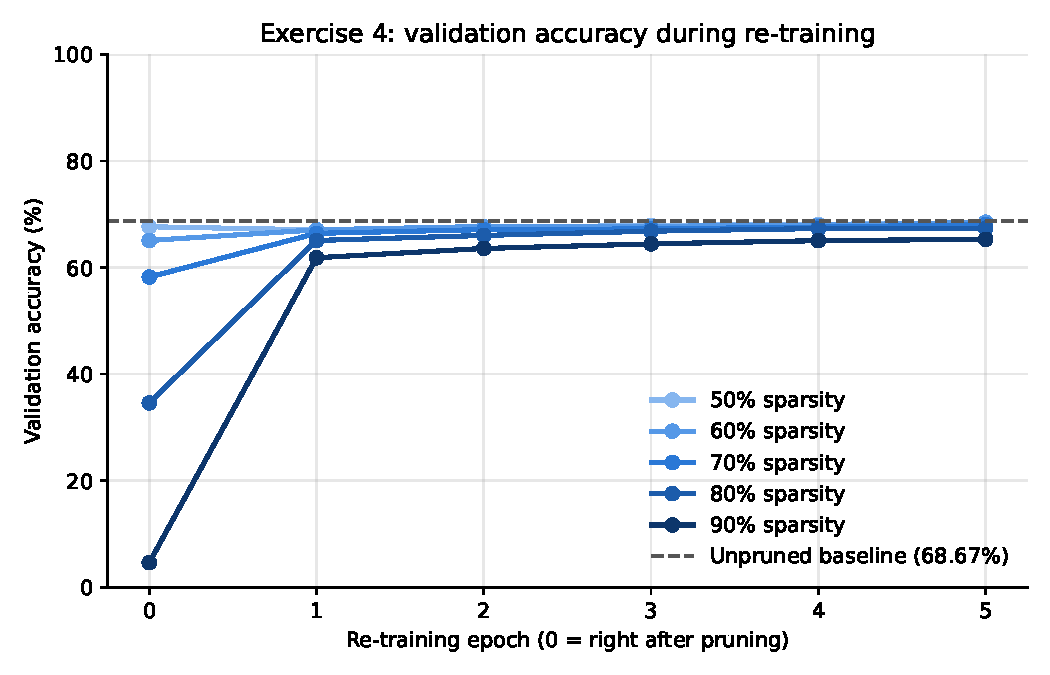
\includegraphics[width=0.62\linewidth]{ex4_retraining_history.pdf}
\caption{Exercise~4: validation accuracy during re-training for the most pruned models (epoch 0 = right after pruning).}
\label{fig:ex4hist}
\end{figure}

\subsection{Comments on the curve}
\textbf{Re-training recovers almost all the lost accuracy}: the curve is nearly flat up to 70\% sparsity, and the 90\% model goes from 4.61\% to 65.31\% with only 10\% of its weights. Most of the recovery happens in the first epoch (34.6\% to 65.1\% at 80\%, Figure~\ref{fig:ex4hist}), which tells me that the surviving weights still hold most of the knowledge and only need to be readjusted.

At low sparsity, re-training seemed to hurt slightly, which I did not expect. \textbf{The control explains it: the unpruned model also loses 0.26 points}, because restarting at learning rate 0.01 moves it away from its converged state and five more epochs add over-fitting. Compared with this control, every pruned model up to 60\% performs the same. Without the control, I would have drawn the wrong conclusion.

\subsection{Which model would I keep, and why?}
\textbf{I would keep the 70\% model after re-training} (68.05\%, 0.62 points below the baseline). It is the sparsest model within my rule, with only 846{,}222 non-zero weights, so re-training moves the usable sparsity from 50\% to 70\%. The 80\% model narrowly misses the rule ($-1.28$) and would be my choice with a slightly larger budget.

% ===========================================================================
\section{Exercise 5: Iterative Training and Pruning}
% ===========================================================================

\subsection{What I implemented}
Following the template's tip, I reused the re-training function of Exercise~4 in a loop. \textbf{I loaded the baseline once and pruned and re-trained the same model six times}, to 20, 40, 60, 70, 80 and 90\% total sparsity, with five epochs after each step. Because PyTorch applies a new pruning amount only to the remaining weights, I computed how many extra weights to remove so that the total reaches the target $s_t$ exactly:
\begin{equation}
  k_t = \operatorname{round}(s_t \cdot N) - \bigl|\{\,i : m_i = 0\,\}\bigr|, \qquad N = 2{,}820{,}740.
\end{equation}
The measured sparsity was exactly the target at every step, and earlier masks were always kept.

\subsection{Results}

\begin{figure}[H]
\centering
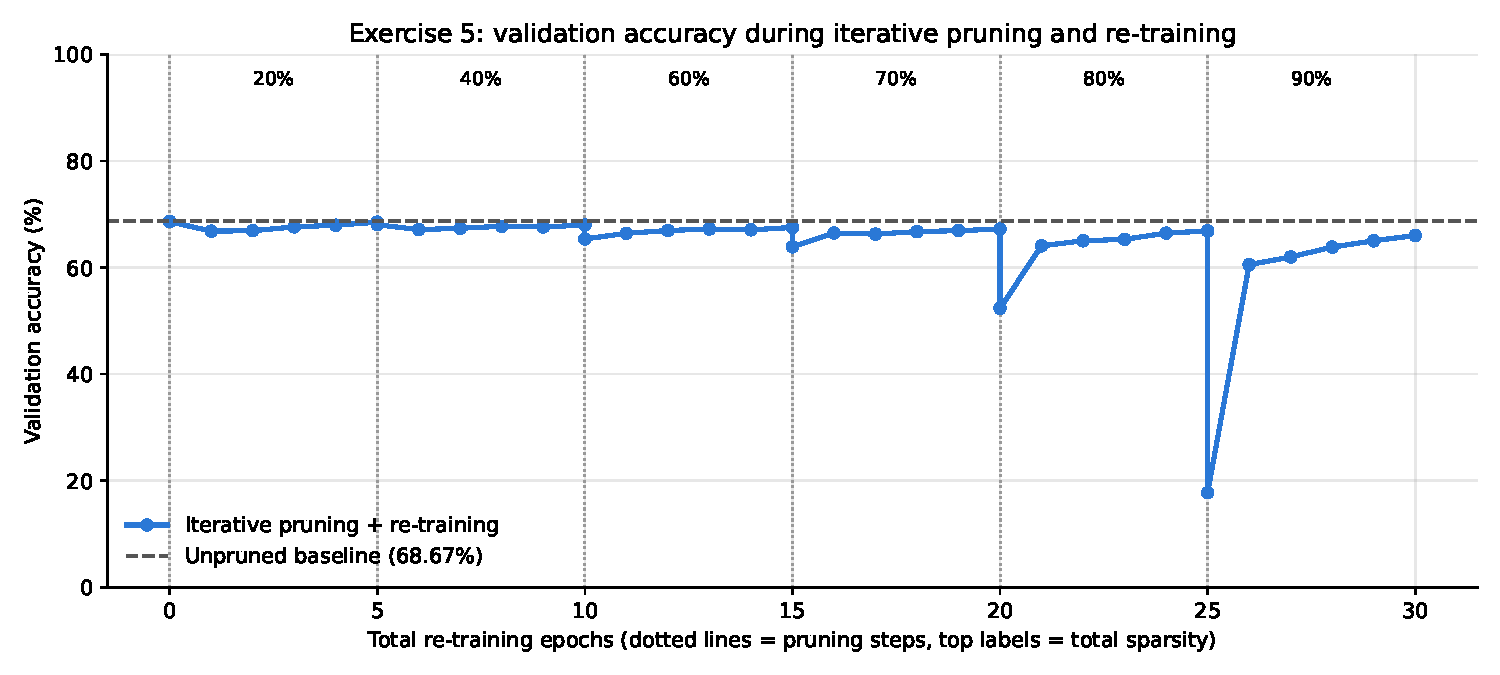
\includegraphics[width=\linewidth]{ex5_iterative_history.pdf}
\caption{Exercise~5: validation accuracy along the iterative procedure (a drop at each pruning step, then recovery).}
\label{fig:ex5hist}
\end{figure}

\begin{figure}[H]
\centering
% Figure 10: Exercise 5, iterative versus one-shot pruning, both after re-training (zoomed axis).
\begin{tikzpicture}
\begin{axis}[report,
  xlabel={Sparsity (\%)}, ylabel={Validation accuracy (\%)},
  xmin=-2, xmax=92, ymin=64.5, ymax=69.5, xtick={0,10,...,90}, legend pos=south west]
\addplot[finetuned, mark=triangle*] table[x=sparsity, y=after]{data/ex4.csv};
\addlegendentry{One-shot + re-training (Ex.~4, 5 epochs)}
\addplot[iterative, mark=diamond*] table[x=sparsity, y=after_retraining]{data/ex5.csv};
\addlegendentry{Iterative + re-training (Ex.~5, $5\times$step epochs)}
\addplot[baseline line] coordinates {(-5,\baselineacc) (95,\baselineacc)};
\addlegendentry{Baseline (68.67\%)}
\node[font=\footnotesize, text=iterative, anchor=west] at (axis cs:38,66.95) {at 60\%: iterative $-0.99$};
\node[font=\footnotesize, text=iterative, anchor=west] at (axis cs:58,65.1) {at 90\%: iterative $+0.72$};
\end{axis}
\end{tikzpicture}

\caption{Exercise~5: iterative versus one-shot pruning, both after re-training (zoomed scale).}
\label{fig:ex5}
\end{figure}

\begin{table}[H]
\centering
\caption{Exercise~5 compared with one-shot pruning. The iterative model at step $t$ received $5t$ epochs of re-training in total; each one-shot model received 5.}
\label{tab:ex5}
\begin{tabular}{rrrrr}
\toprule
 & \multicolumn{2}{c}{After pruning} & \multicolumn{2}{c}{After re-training} \\
\cmidrule(lr){2-3}\cmidrule(lr){4-5}
Sparsity & One-shot & Iterative & One-shot & Iterative \\
\midrule
20\% & 68.61\% & 68.61\% & 68.51\% & 68.52\% \\
40\% & 68.21\% & 68.05\% & 68.66\% & \textbf{67.99\%} \\
60\% & 65.09\% & 65.37\% & 68.52\% & 67.53\% \\
70\% & 58.22\% & 63.90\% & 68.05\% & 67.23\% \\
80\% & 34.60\% & 52.37\% & 67.39\% & 66.88\% \\
90\% & 4.61\% & 17.75\% & 65.31\% & 66.03\% \\
\bottomrule
\end{tabular}
\end{table}

\subsection{Comments on the curve}
As I expected, \textbf{each pruning step is much less damaging when the network has been pruned progressively}: right after reaching 80\%, the iterative model keeps 52.4\% accuracy instead of 34.6\%, and 17.8\% instead of 4.6\% at 90\%. However, \textbf{after re-training, iterative pruning only beats one-shot pruning at 90\%} ($+0.72$ points); between 40\% and 80\% it ends 0.5--1.0 point below. The 20\% step is identical to Exercise~4 and gives the same result, which rules out an implementation error.

\textbf{My explanation is accumulated over-fitting.} The model is re-trained again and again on the same images (30 epochs in total at 90\%): its training accuracy reaches about 99.5\% at steps 3--4, while its validation loss rises from 1.24 to 1.40, against about 1.22 for the one-shot models. At 90\% the network is too small to memorise as much, and the gradual approach finally pays off. I did not confirm this with a dedicated experiment, for example with fewer epochs per step.

\subsection{Which model would I keep, and why?}
My rule selects the \textbf{iterative 40\% model} (67.99\%). However, the one-shot 70\% model of Exercise~4 is sparser, more accurate and cheaper to obtain, so \textbf{it remains my overall choice}. Iterative pruning would be my choice only for very high compression (90\%).

% ===========================================================================
\section{Final Evaluation on the Test Set}
% ===========================================================================

Once all choices were fixed, I evaluated the selected models once on the official test set with \code{evaluate.py} (Table~\ref{tab:final}, Figure~\ref{fig:final}).

\begin{table}[H]
\centering
\caption{Final evaluation. All models were selected beforehand on the validation set.}
\label{tab:final}
\resizebox{\linewidth}{!}{%
\begin{tabular}{lrrrr}
\toprule
Model & Sparsity & Non-zero params & Val.\ acc. & \textbf{Test acc.} \\
\midrule
Baseline (Ex.~0) & 0\% & 2{,}820{,}740 & 68.67\% & \textbf{68.54\%} \\
Global, no re-training (Ex.~3) & 50\% & 1{,}410{,}370 & 67.67\% & 67.37\% \\
\textbf{Global + re-training (Ex.~4), final} & \textbf{70\%} & \textbf{846{,}222} & 68.05\% & \textbf{68.34\%} \\
Global + re-training (Ex.~4) & 80\% & 564{,}148 & 67.39\% & 67.84\% \\
Iterative (Ex.~5) & 40\% & 1{,}692{,}444 & 67.99\% & 67.76\% \\
Iterative (Ex.~5) & 90\% & 282{,}074 & 66.03\% & 66.09\% \\
\bottomrule
\end{tabular}}
\end{table}

\begin{figure}[H]
\centering
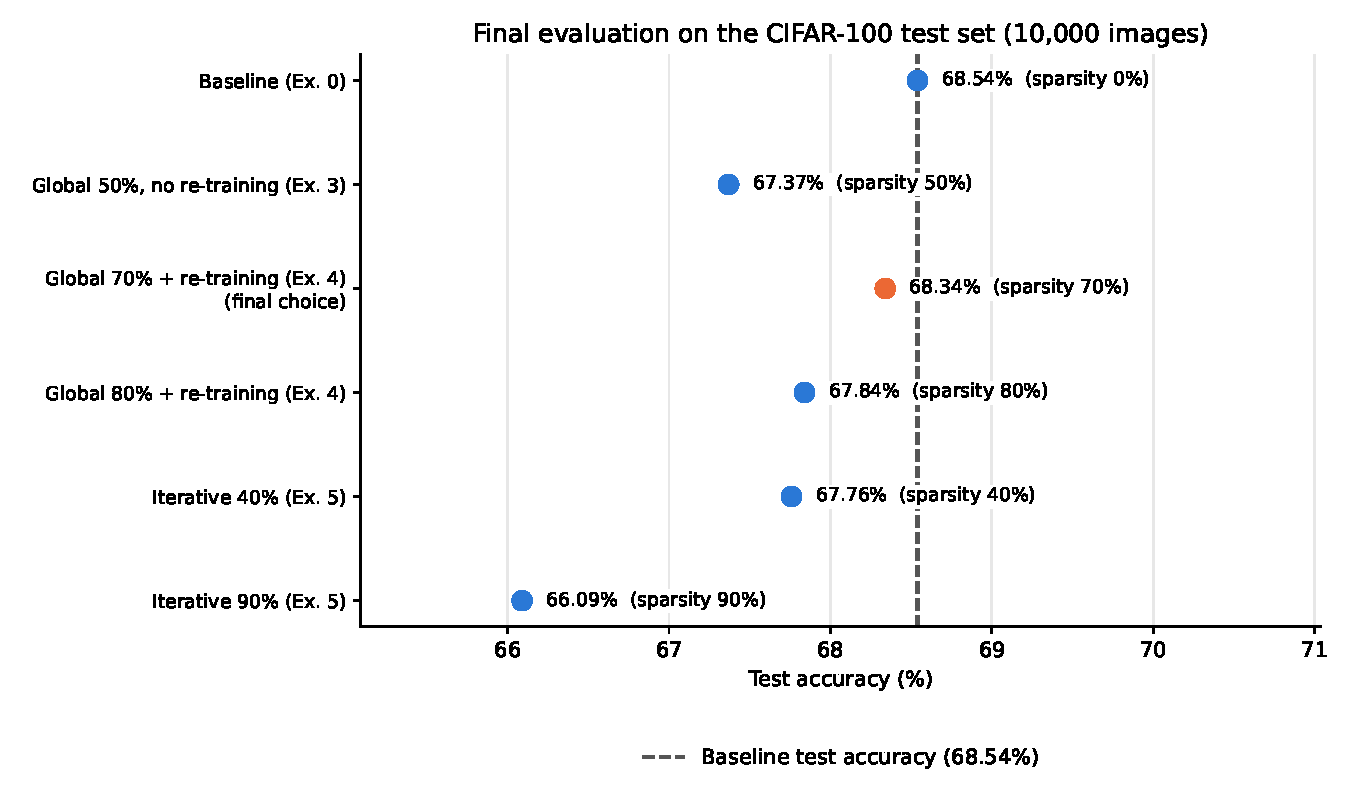
\includegraphics[width=0.8\linewidth]{final_test_accuracy.pdf}
\caption{Test accuracy of the selected models (the final choice in orange).}
\label{fig:final}
\end{figure}

\textbf{My final model keeps only 30\% of its weights and reaches 68.34\% on the test set, 0.20 points below the baseline} (20 images out of 10{,}000). For every model, test and validation accuracy differ by less than 0.5 points, so the selection on the validation set was reliable and the conclusions of the exercises hold on new data. The 80\% model is within one point on the test set ($-0.70$) although it missed my rule on validation; \textbf{I deliberately did not switch to it}, because choosing a model by its test score would make the reported result optimistic.

% ===========================================================================
\section{Bonus: A Custom Structured Pruning Method}
% ===========================================================================

\subsection{Motivation}
In every exercise so far, the zeros did not make the model smaller or faster, because the tensors keep their shape. The bonus asks for my own method inheriting from \code{BasePruningMethod}, removing the \code{amount} lowest structures by L1 norm for weights with more than two dimensions. \textbf{I chose to remove whole filters (output channels) of each convolution}, following Li et al.~\cite{li2017pruning}, because a zero filter could actually be removed from the network.

\subsection{Implementation}
For each filter $j$, the importance is its L1 norm $\|F_j\|_1 = \sum_{c,u,v} |W_{j,c,u,v}|$; the \code{amount} fraction of filters with the smallest norm get their whole mask set to zero, and tensors with two dimensions or fewer are left unchanged:

\noindent\begin{minipage}{\linewidth}
\begin{lstlisting}
def compute_mask(self, t, default_mask):
    mask = default_mask.clone()
    if t.dim() <= 2:
        return mask  # only weights with dimensionality > 2 are pruned
    filter_norms = (t * default_mask).abs().sum(dim=tuple(range(1, t.dim())))
    n_pruned = round(self.amount * t.shape[0])
    if n_pruned > 0:
        pruned_filters = torch.topk(filter_norms, k=n_pruned, largest=False).indices
        mask[pruned_filters] = 0  # the whole filter is set to zero
    return mask
\end{lstlisting}
\end{minipage}

I applied it layer by layer to all 20 convolutions (2{,}400 filters) at 0--50\%, then re-trained each model with the function of Exercise~4. The number of zero filters was exactly as expected and unchanged after re-training.

\subsection{Results}

\begin{figure}[H]
\centering
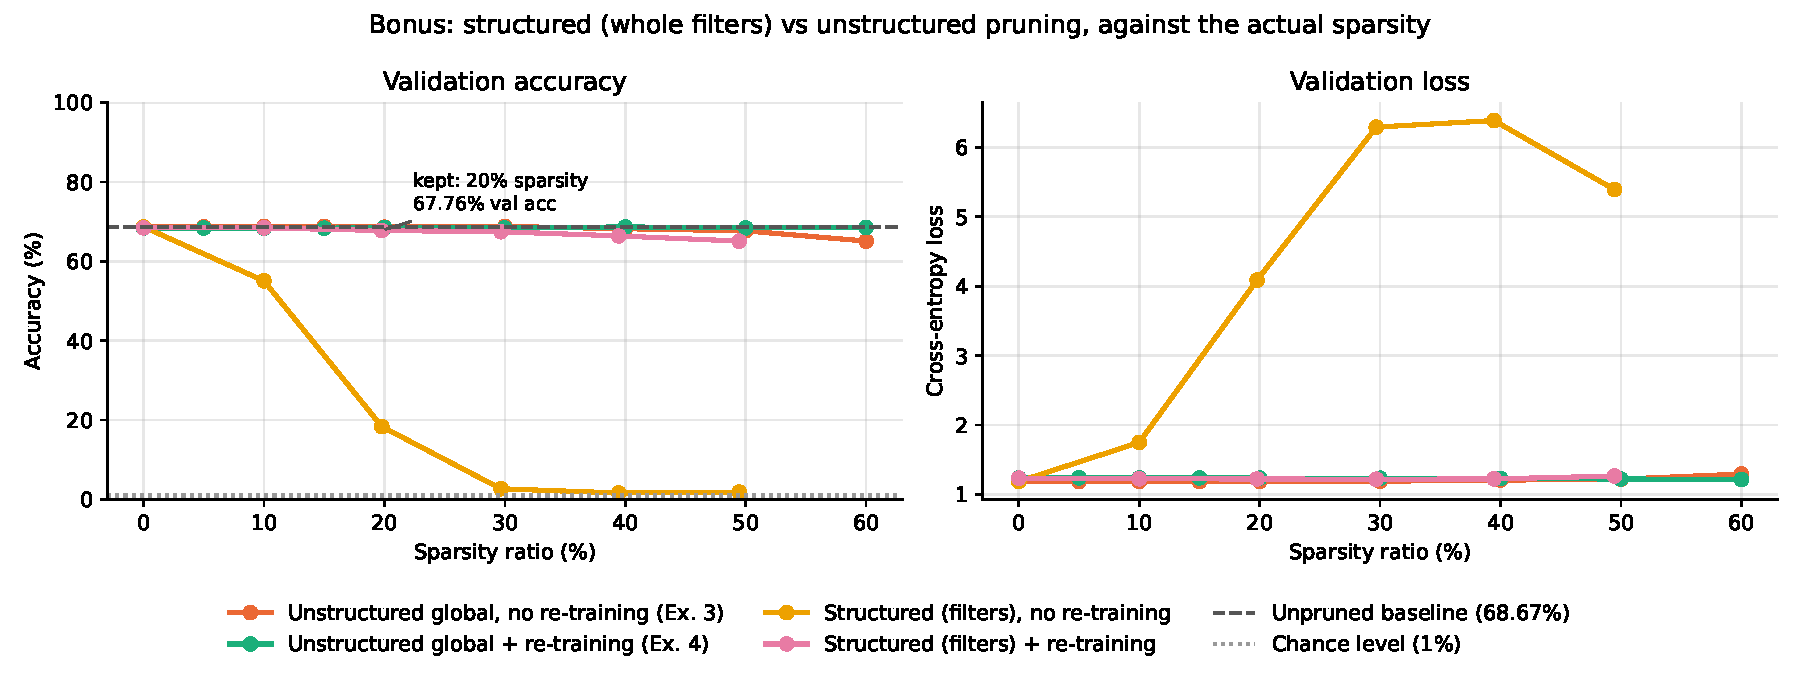
\includegraphics[width=\linewidth]{bonus_curve.pdf}
\caption{Bonus: structured (whole filters) versus unstructured pruning, before and after re-training.}
\label{fig:bonus}
\end{figure}

\begin{table}[H]
\centering
\caption{Bonus: structured filter pruning compared with unstructured global pruning (validation set).}
\label{tab:bonus}
\resizebox{\linewidth}{!}{%
\begin{tabular}{rrrrr}
\toprule
Filters removed & Actual sparsity & Structured, no re-train & Structured + re-train & Unstructured + re-train (Ex.~4) \\
\midrule
10\% & 10.00\% & 55.06\% & 68.42\% & 68.35\% \\
\textbf{20\%} & 19.78\% & 18.37\% & \textbf{67.76\%} & 68.51\% \\
30\% & 29.68\% & 2.70\% & 67.45\% & 68.40\% \\
50\% & 49.46\% & 1.87\% & 65.08\% & 68.41\% \\
\bottomrule
\end{tabular}}
\end{table}

\subsection{Discussion}
\textbf{Without re-training, structured pruning is far more destructive than unstructured pruning}: a filter with a small total norm can still contain large useful weights, and removing it deletes a whole feature map. Re-training recovers most of the accuracy: with 10\% of the filters removed the model matches the re-trained control, and \textbf{with 20\% it stays within my rule (67.76\%)}. It remains below unstructured pruning at the same sparsity, and the gap grows to 3.3 points at 50\%, which is the price of structure.

\textbf{The advantage is that these zeros form complete channels}, which could be physically removed to obtain a genuinely smaller and faster network. I did not implement this removal, because it requires handling the residual connections and the batch-norm shifts, so I do not claim any measured speed-up. My kept structured model is the one with 20\% of the filters removed.

% ===========================================================================
\section{Overall Discussion}
% ===========================================================================

\begin{table}[H]
\centering
\caption{Summary: highest sparsity of each method within one point of the baseline (validation), and its test accuracy when evaluated.}
\label{tab:summary}
\resizebox{\linewidth}{!}{%
\begin{tabular}{lrrrl}
\toprule
Method & Kept sparsity & Val.\ acc. & Test acc. & Re-training \\
\midrule
Baseline & 0\% & 68.67\% & 68.54\% & -- \\
Layer-by-layer L1 (Ex.~2) & 0\% & 68.67\% & -- & none \\
Global L1 (Ex.~3) & 50\% & 67.67\% & 67.37\% & none \\
\textbf{Global L1 + re-training (Ex.~4)} & \textbf{70\%} & \textbf{68.05\%} & \textbf{68.34\%} & 5 epochs \\
Iterative global L1 (Ex.~5) & 40\% & 67.99\% & 67.76\% & 10 epochs in total \\
Structured, filters (Bonus) & 20\% (filters) & 67.76\% & -- & 5 epochs \\
\bottomrule
\end{tabular}}
\end{table}

Looking back at Table~\ref{tab:summary}, \textbf{the most important lesson for me is that where the weights are removed matters more than how many}: the same L1 criterion destroys the network layer by layer but removes half of the weights for less than one point globally. \textbf{Re-training is part of the method}, since five epochs moved the usable sparsity from 50\% to 70\%. I also learned that \textbf{a control experiment can change the conclusion completely}, and that \textbf{a more elaborate method is not automatically better}: my iterative schedule was gentler, yet the simpler one-shot approach won almost everywhere. Finally, \textbf{sparsity is not compression}: only structured pruning produces zeros that can actually be exploited.

These results have limitations. They come from a single run and a single seed, so differences below about half a point are within noise; I tested only one re-training setting; the one-point rule is my own choice; my explanations about batch normalisation and over-fitting were not confirmed by dedicated experiments; and the structured model was not physically shrunk.

% ===========================================================================
\section{Conclusion}
% ===========================================================================

In this lab I implemented and compared the main magnitude-based pruning procedures on a ResNet-18-like network trained on CIFAR-100. Layer-by-layer pruning was very harmful, global pruning kept the accuracy up to 50\% sparsity without re-training, and \textbf{global pruning followed by a short re-training gave the best result: 70\% of the weights removed for 68.34\% test accuracy}, only 0.20 points below the baseline. Iterative pruning reduced the damage of each step but only helped at 90\%, and my structured method showed the trade-off between accuracy and exploitable sparsity. I started this lab with the simple idea that ``small weights are useless'', and I end it with a more nuanced view: the importance of a weight depends on its layer, re-training is part of the method, every comparison needs a fair control, and the type of sparsity decides whether pruning brings any practical benefit.

% ===========================================================================
\begin{thebibliography}{99}

\bibitem{han2015learning}
S.~Han, J.~Pool, J.~Tran, and W.~J. Dally.
\newblock Learning both weights and connections for efficient neural network.
\newblock In \emph{Advances in Neural Information Processing Systems (NIPS)}, 2015.

\bibitem{li2017pruning}
H.~Li, A.~Kadav, I.~Durdanovic, H.~Samet, and H.~P. Graf.
\newblock Pruning filters for efficient ConvNets.
\newblock In \emph{International Conference on Learning Representations (ICLR)}, 2017.

\bibitem{zhu2017prune}
M.~Zhu and S.~Gupta.
\newblock To prune, or not to prune: exploring the efficacy of pruning for model compression.
\newblock \emph{arXiv preprint arXiv:1710.01878}, 2017.

\bibitem{he2016deep}
K.~He, X.~Zhang, S.~Ren, and J.~Sun.
\newblock Deep residual learning for image recognition.
\newblock In \emph{IEEE Conference on Computer Vision and Pattern Recognition (CVPR)}, 2016.

\bibitem{he2015delving}
K.~He, X.~Zhang, S.~Ren, and J.~Sun.
\newblock Delving deep into rectifiers: surpassing human-level performance on ImageNet classification.
\newblock In \emph{IEEE International Conference on Computer Vision (ICCV)}, 2015.

\bibitem{ioffe2015batch}
S.~Ioffe and C.~Szegedy.
\newblock Batch normalization: accelerating deep network training by reducing internal covariate shift.
\newblock In \emph{International Conference on Machine Learning (ICML)}, 2015.

\bibitem{loshchilov2017sgdr}
I.~Loshchilov and F.~Hutter.
\newblock SGDR: stochastic gradient descent with warm restarts.
\newblock In \emph{International Conference on Learning Representations (ICLR)}, 2017.

\bibitem{krizhevsky2009learning}
A.~Krizhevsky.
\newblock Learning multiple layers of features from tiny images.
\newblock Technical report, University of Toronto, 2009.

\bibitem{paszke2019pytorch}
A.~Paszke et~al.
\newblock PyTorch: an imperative style, high-performance deep learning library.
\newblock In \emph{Advances in Neural Information Processing Systems (NeurIPS)}, 2019.

\bibitem{paganini2019pruning}
M.~Paganini.
\newblock Pruning tutorial.
\newblock PyTorch Tutorials, \url{https://pytorch.org/tutorials/intermediate/pruning_tutorial.html}.

\end{thebibliography}

% ===========================================================================
\appendix
\section{Per-layer Sparsity of the Kept Global Model (Exercise 3, 50\%)}
\label{app:layers}

\begin{table}[H]
\centering
\small
\caption{Sparsity of every layer of the global 50\% model (weights and biases counted together).}
\resizebox{\linewidth}{!}{%
\begin{tabular}{llrr@{\hskip 2.5em}llrr}
\toprule
Layer & Type & Params & Sparsity & Layer & Type & Params & Sparsity \\
\midrule
stem.0 & Conv & 864 & 9.26\% & layer3.0.conv1 & Conv & 73{,}728 & 33.61\% \\
stem.1 & BN & 64 & 3.12\% & layer3.0.bn1 & BN & 256 & 4.30\% \\
layer1.0.conv1 & Conv & 9{,}216 & 37.70\% & layer3.0.conv2 & Conv & 147{,}456 & 37.95\% \\
layer1.0.bn1 & BN & 64 & 1.56\% & layer3.0.bn2 & BN & 256 & 7.81\% \\
layer1.0.conv2 & Conv & 9{,}216 & 33.57\% & layer3.0.shortcut.0 & Conv & 8{,}192 & 20.51\% \\
layer1.0.bn2 & BN & 64 & 6.25\% & layer3.0.shortcut.1 & BN & 256 & 8.20\% \\
layer1.1.conv1 & Conv & 9{,}216 & 33.91\% & layer3.1.conv1 & Conv & 147{,}456 & 43.45\% \\
layer1.1.bn1 & BN & 64 & 10.94\% & layer3.1.bn1 & BN & 256 & 0.00\% \\
layer1.1.conv2 & Conv & 9{,}216 & 31.45\% & layer3.1.conv2 & Conv & 147{,}456 & 47.54\% \\
layer1.1.bn2 & BN & 64 & 4.69\% & layer3.1.bn2 & BN & 256 & 2.73\% \\
layer2.0.conv1 & Conv & 18{,}432 & 34.50\% & layer4.0.conv1 & Conv & 294{,}912 & 45.20\% \\
layer2.0.bn1 & BN & 128 & 3.12\% & layer4.0.bn1 & BN & 512 & 0.20\% \\
layer2.0.conv2 & Conv & 36{,}864 & 34.69\% & layer4.0.conv2 & Conv & 589{,}824 & 53.43\% \\
layer2.0.bn2 & BN & 128 & 7.03\% & layer4.0.bn2 & BN & 512 & 0.00\% \\
layer2.0.shortcut.0 & Conv & 2{,}048 & 13.72\% & layer4.0.shortcut.0 & Conv & 32{,}768 & 27.28\% \\
layer2.0.shortcut.1 & BN & 128 & 7.03\% & layer4.0.shortcut.1 & BN & 512 & 0.00\% \\
layer2.1.conv1 & Conv & 36{,}864 & 32.23\% & layer4.1.conv1 & Conv & 589{,}824 & 50.32\% \\
layer2.1.bn1 & BN & 128 & 0.00\% & layer4.1.bn1 & BN & 512 & 0.00\% \\
layer2.1.conv2 & Conv & 36{,}864 & 34.97\% & layer4.1.conv2 & Conv & 589{,}824 & 64.44\% \\
layer2.1.bn2 & BN & 128 & 3.91\% & layer4.1.bn2 & BN & 512 & 0.98\% \\
 & & & & fc & Linear & 25{,}700 & 9.77\% \\
\bottomrule
\end{tabular}}
\end{table}

\section{Reproducing the Results}
All commands are run from the lab directory, in the \code{PyTorch} conda environment. Each exercise in \code{pruning.py} is selected with the \code{run\_exercises} list at the top of the file and writes its models, CSV files, log and figures to \code{results/<exercise>/}.

\begin{lstlisting}[language=bash]
python train.py                 # Exercise 0 (baseline, ~9 min on an RTX 4060 laptop GPU)
python pruning.py               # with run_exercises = [1], [2], [3], [4], [5] or ["bonus"]
python evaluate.py              # final evaluation of the selected models (val + test)
python evaluate.py results/exercise4/exercise4_finetuned_70.pt --split test   # a single model
\end{lstlisting}

\end{document}
